\chapter{温度や湿度、明るさを測ってみよう}
\section{この章で学ぶこと}
この章では以下のことを学びます。

\begin{itemize}
  \item コンピュータをコマンドを使って動かす
  \item ファイルとディレクトリを文字で指定する
  \item センサーボードをプログラムで動かす
  \begin{itemize}
    \item LEDの点灯・消灯
    \item 温湿度気圧センサーの値を読む
    \item ボタンを上手に使う
  \end{itemize}
\end{itemize}

まずコンピュータをコマンドで動かす方法を学びます。
マウスではなく、コマンドでコンピュータを操作することは、とても重要です。
コマンドを使うと、コンピュータがするべき操作を文字で記録したり、
離れたコンピュータを簡単に操作できるようになります。
また、コマンドでファイルを扱うために、ファイルが置いてある場所を指示する方法を学びます。
ターミナルを利用して、文字を使ってファイルの操作をできるようになりましょう。

次に、センサーボードをプログラムから動かす方法を学びます。
センサーボードに取り付けてあるLEDを点灯・消灯させたり、
温湿度気圧センサーの情報を読み取ったり、ボタンを上手に使ったりして、
センサーボードをプログラムから動かすことができるようになりましょう。

\section{ターミナルを使ってみよう}
\subsection{コマンドについて知ろう}

ターミナルではコマンドを使ってコンピュータとやりとりをします。
コマンドとはコンピュータにあたえる命令のことです。
コマンドは下のようなかたちで書きます。

\begin{description}
\item[コマンド\textvisiblespace オプション\textvisiblespace \ruby{引数}{ひき|すう}1\textvisiblespace 
\ruby{引数}{ひき|すう}2]\mbox{}\\
 コマンドは動作、引数はそうさのたいしょうです。
 コマンドの最後にEnterキー(エンターキー)を押して、
 コンピュータにコマンドを送ります。
 EnterキーはReturn(リターン)キーと呼ぶこともあります。
\end{description}

使うときは次のことに気を付けましょう。
\begin{itemize}
\item \emph{半角英数字でかくこと}
\item \emph{間にスペース(空白)をいれること}
\end{itemize}

今回はわかりやすいように、スペースを「\textvisiblespace 」のように示しました。
次回からはこのようにしません。どこにスペースを入れるべきかをしっかり覚えましょう。

みなさんが使うラズパイでは英語が使われています。最初から入っているフォルダの名前も英語になっています。
読み方を知りたい人は\pageref{英語と日本語の対応表}ページの英語と日本語の対応表を見てみましょう。

\subsection{自分がどのディレクトリにいるかしろう}
ディレクトリとは、第1回で習ったフォルダと基本的に同じものです。
マウスで操作する場合はフォルダ、コマンドで操作する場合はディレクトリと呼ぶことが多いです。

\begin{description}
\item[pwd]\mbox{}\\
 カレントディレクトリ(自分が今いるディレクトリ)が表示されます。
\end{description}

\begin{lstlisting}[caption=pwdコマンドの例,label=pwdtest]
<#green#pi@raspberrypi#>:<#blue#~ $#> pwd
/home/pi   <-- カレントディレクトリが表示されます
<#green#pi@raspberrypi#>:<#blue#~ $#>
\end{lstlisting}

\begin{tcolorbox}[title=\useOmetoi]
\begin{enumerate}
 \item 実際にpwdを使って、カレントディレクトリが表示されることを確かめましょう。
 表示されたカレントディレクトリを書いてください。\\
\underline{答え.\hspace{0.8\linewidth}}
\end{enumerate}
\end{tcolorbox}



\subsection{ディレクトリの中を見てみよう}
\begin{description}
\item[ls\textvisiblespace -F\textvisiblespace ディレクトリ]\mbox{}\\
ディレクトリの中のファイルやディレクトリが表示されます。
ファイルはピンクの文字、ディレクトリは青い文字になっています。
\end{description}

%//terminal[lsF-test][ls -F コマンドの例]{
\begin{lstlisting}[caption=ls -F コマンドの例,label=lsFtest]
<#green#pi@raspberrypi#>:<#blue#~ $#> ls -F
<#blue#MagPi/  ダウンロード/ デスクトップ/  ビデオ/ 画像/
ome/   テンプレート/  ドキュメント/  音楽/   公開/#> <--ファイルやディレクトリが表示されます
<#green#pi@raspberrypi#>:<#blue#~ $#>
\end{lstlisting}

\begin{itemize}
\item[<例>] ls\textvisiblespace -Fだけを入力するとカレントディレクトリの中を見ることができます。 
\item[<例>] Picturesというディレクトリの中を見たい場合は ls\textvisiblespace -F\textvisiblespace Pictures/と入力します。 
\end{itemize}

ディレクトリの中にあるファイルは人によってちがいます。
\begin{lstlisting}[caption=ls -F Pictures/コマンドの例,label=lsFPicttest]
<#green#pi@raspberrypi#>:<#blue#~ $#> ls -F Pictures
<#magenta#2019-07-08-145604_1366X768_scrot.png  2019-07-08-150326_1366X768_scrot.png  
2019-07-08-150313_1366X768_scrot.png  2019-07-08-150348_1366X768_scrot.png  
2019-07-08-150323_1366X768_scrot.png  2019-07-08-150356_1366X768_scrot.png  #>
<#green#pi@raspberrypi#>:<#blue#~ $#> 
\end{lstlisting}

\begin{tcolorbox}[title=\useOmetoi]
\begin{enumerate}
\item ls\textvisiblespace -Fと入力して出てきたファイルとディレクトリの名前を1つずつ書きましょう。\\
\underline{答え.\hspace{0.8\linewidth}}
\item ls\textvisiblespace -F\textvisiblespace Pictures/ と入力して出てきたファイルかディレクトリの名前を1つ書きましょう。\\
\underline{答え.\hspace{0.8\linewidth}}
\end{enumerate}
\end{tcolorbox}




\section{ファイルとディレクトリ}
\subsection{ファイル、ディレクトリってなんだろう?}
ファイルはコンピュータに保存されている文章、画像、音楽などのデータです。
多くの場合、人間はコンピュータにファイルを操作させることで仕事をします。
ファイルには「\ruby{拡張子}{かく|ちょう|し}」がついており、
そのファイルがどんな種類なのかを表します。
たとえば、画像ファイルを表す.jpgや、動画ファイルを表す.mp4、
テキストファイルを表す.txtなどがあります。

\begin{table}[H]
  \begin{center}
    \caption[tab:files]{ファイルの種類}
    \begin{tabular}{|c|c|c|} \hline
    \begin{minipage}{0.3\hsize}
      \begin{center}
        
\includegraphics[width=\linewidth]{images/chap03/text03-img001.png}
      \end{center}  
    \end{minipage} & 
    \begin{minipage}{0.3\hsize}
      \begin{center}
        
\includegraphics[width=\linewidth]{images/chap03/text03-img002.png}
      \end{center}
    \end{minipage} &
    \begin{minipage}{0.3\hsize}
      \begin{center}
        
\includegraphics[width=\linewidth]{images/chap03/text03-img003.png}
      \end{center} 
    \end{minipage} \\ \hline
    oto.mp3 & gazou.jpg & douga.mp4 \\ \hline
  \end{tabular}
 \end{center}
\end{table}


ディレクトリとはファイルを分類・整理するためのもので、
いくつかのファイルを入れておくためのファイルです。
ファイルを紙だとしてディレクトリはバインダーだと思うとわかりやすいでしょう。

\begin{tcolorbox}[title=\useOmetoi]
\begin{enumerate}
\item ファイルとはなんでしょうか。\\
\underline{答え.\hspace{0.8\linewidth}}
\item ディレクトリとはなんでしょうか。\\
\underline{答え.\hspace{0.8\linewidth}}
\item どんな拡張子があるかインターネットで調べてみましょう。
\end{enumerate}

\begin{table}[H]
  \centering
  \begin{tabular}{lrr} \toprule
番号 & 拡張子 & 表すもの \\ \midrule
1. & .jpg & 画像 \\
2. & .mp4 & 動画 \\
3. & \hspace{10\zw} & \hspace{10\zw} \\
4. & \hspace{10\zw} & \hspace{10\zw} \\
5. & \hspace{10\zw} & \hspace{10\zw} \\ \bottomrule
\end{tabular}
\end{table}
例を見て、拡張子とその拡張子が何を表すか2つ書いてみましょう。
\end{tcolorbox}

\subsection{ディレクトリの関係}
いま注目しているディレクトリの中に入っているディレクトリを\emph{下のディレクトリ}、
いま注目しているディレクトリを中に持っているディレクトリを\emph{上のディレクトリ}と呼びます。

一番上のディレクトリは / スラッシュで書きます。その下にあるbin boot dev etcなどのディレクトリはコンピュータの設定ファイルを持っているので、間違った使い方をすると壊れます。気を付けましょう。

ユーザが作業に使ってもよいディレクトリを\emph{ホームディレクトリ}と言います。
ユーザの作業はホームディレクトリの下で行います。
ホームディレクトリは、ラズベリーパイでは\emph{/home/あなたのユーザ名}です。
ホームディレクトリを示すために記号「\textasciitilde」(チルダ)を使うこともできます。

みなさんが今、作業に使っているディレクトリは\emph{カレントディレクトリ}と言います。
カレントディレクトリは./と書くことができます。
カレントディレクトリから一つ上のディレクトリは../と書くことができます。
ディレクトリは/で区切ります。

ディレクトリの位置は\emph{一番上のディレクトリ(/)から見てどこにあるか(絶対パス)}、
または\emph{カレントディレクトリから見てどこにあるか(相対パス)}で決まります。
絶対パスの特徴は\emph{パスの先頭に / がついています}。相対パスの特徴は\emph{パスの先頭に / がついていません}。

\textasciitilde から始まるディレクトリの位置は、\textasciitilde を
「/home/あなたのユーザ名」と置き換えたものとして扱われます。

カレントディレクトリにあるディレクトリxxxの位置を指定する場合は、
xxx、xxx/、./xxx、./xxx/などと書きます。いろいろな指定の仕方があるのは面白いですね。

ホームディレクトリにあるファイルyyyの位置を指定する場合は、
\textasciitilde /yyy, または /home/あなたのユーザ名/yyy と書きます。ファイルの後ろにはスラッシュ記号(/)はつけません。

図\ref{fig:folder-path}にユーザー名が「pi」のときのフォルダとフォルダの関係をパスであらわしてあります。
パスとフォルダ間の関係を考えながら図を読みましょう。

\begin{figure}[H]
    \begin{minipage}{0.4\hsize}
        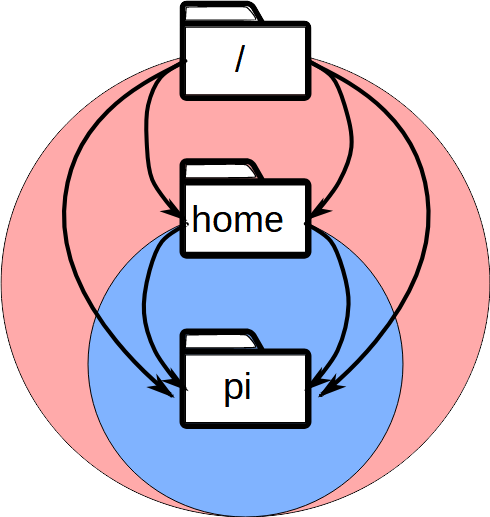
\includegraphics[width=\hsize]{images/chap03/text03-img004.png}
    \end{minipage}
    \begin{minipage}{0.6\hsize}
        \begin{itemize}
        \item /は一番上のディレクトリから見ると/
        \item /はカレントディレクトリが/のとき./
        \item /はカレントディレクトリがhomeのとき../
        \item /はカレントディレクトリがpiのとき../../
        \item homeは一番上のディレクトリから見ると/home
        \item homeはカレントディレクトリが/のとき./home
        \item homeはカレントディレクトリがhomeのとき./
        \item homeはカレントディレクトリがpiのとき../
        \item piは一番上のディレクトリから見ると/home/pi
        \item piはカレントディレクトリが/のとき./home/pi
        \item piはカレントディレクトリがhomeのとき./pi
        \item piはカレントディレクトリがpiのとき./
        \end{itemize}
    \end{minipage}
    \caption{フォルダ間の関係をパスで説明する}
    \label{fig:folder-path}
\end{figure}

\begin{tcolorbox}[title=\useOmetoi]
\begin{figure}[H]
 \centering
 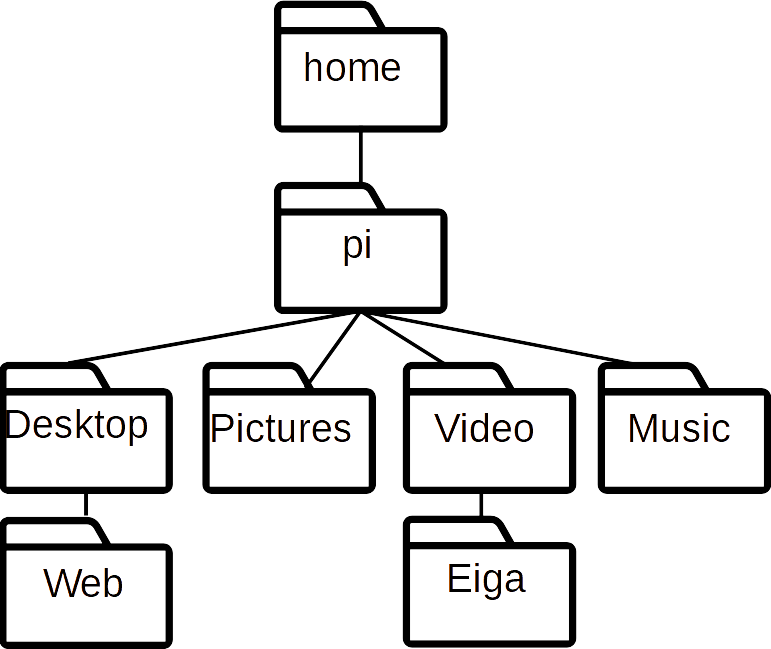
\includegraphics[width=0.6\linewidth]{images/chap03/text03-img005.png}
\end{figure}
ユーザー名を「pi」としたときに以下の問題に答えてみましょう。
\begin{enumerate}
\item ホームディレクトリはどれでしょうか\\
\underline{答え.\hspace{0.8\linewidth}}
\item カレントディレクトリが/home/pi/Videoのとき、上のディレクトリはどれでしょうか。\\
\underline{答え.\hspace{0.8\linewidth}}
\item カレントディレクトリが/home/piのとき、下のディレクトリはどれでしょうか。4つあります。\\
\underline{答え.\hspace{0.8\linewidth}}
\item カレントディレクトリが/home/pi/Desktopのとき、上のディレクトリはどれでしょうか。\\
\underline{答え.\hspace{0.8\linewidth}}
\item カレントディレクトリが\textasciitilde /Desktopのとき、下のディレクトリはどれでしょうか。\\
\underline{答え.\hspace{0.8\linewidth}}
\end{enumerate}
\end{tcolorbox}
 
